%%%%%%%%%%%%%%%%%%%%%%%%%%%%%%%%%%%%%%%%%
% Design based on a template by Roberto and following the format of
% the xmipp tutorials. In turn, they seem to be based on a template
% from http://www.latextemplates.com
%%%%%%%%%%%%%%%%%%%%%%%%%%%%%%%%%%%%%%%%%

%----------------------------------------------------------------------------------------
%	PACKAGES AND OTHER DOCUMENT CONFIGURATIONS
%----------------------------------------------------------------------------------------

\documentclass[12pt]{article} % Default font size is 12pt, it can be changed here
\usepackage[english]{babel}
\usepackage[utf8]{inputenc}
\usepackage{listings} % To include source code
\usepackage{caption}
\usepackage{geometry} % Required to change the page size to A4
%\geometry{a4paper} % Set the page size to be A4 as opposed to the default US Letter
\usepackage{framed}
\usepackage{url}
\usepackage{graphicx} % Required for including pictures
\usepackage{natbib}
\usepackage{float} % Allows putting an [H] in \begin{figure} to specify the exact location of the figure
\usepackage{hyperref}
\usepackage{menukeys}

\usepackage{fancyhdr}
\pagestyle{fancy}
\fancyhf{}
\fancyhead[RO]{{Mix-and-Match Tutorial}}
\fancyhead[LO]{Scipion}
%\fancyhead[RO]{{\leftmark}}
\fancyfoot[RO]{\thepage}

\linespread{1.2} % Line spacing

%\setlength\parindent{0pt} % Uncomment to remove all indentation from paragraphs

\newcommand{\scipion}{\textsc{Scipion} }
\newcommand{\tipnote}[1]{\begin{description}\item \textbf{NOTE}  #1\end{description}}
                                                           
\newenvironment{command}{\tt\begin{quote}}{\end{quote}}
\newcommand{\comm}[1]{\texttt{#1}}

\begin{document}


%----------------------------------------------------------------------------------------
%	TITLE PAGE
%----------------------------------------------------------------------------------------

\begin{titlepage}

% New command for horizontal lines. Change thickness here.
\newcommand{\HRule}{\rule{\linewidth}{0.5mm}}

\center % Center everything on the page


\includegraphics{../tutorial_common/images/scipion_logo.png}

{\large Scipion Tutorial Series}\\[1.0cm]

\textsc{\LARGE National Center for Biotechnology}\\[0.5cm]
\textsc{\Large Biocomputing Unit}\\[0.5cm]

\HRule\\[0.4cm]
{ \huge \bfseries Mix-and-Match Tutorial}\\[0.4cm] % Title of your document
\HRule \\[1.5cm]

%{\large \today}\\[3cm] % Date, change the \today to a set date if you want to be precise

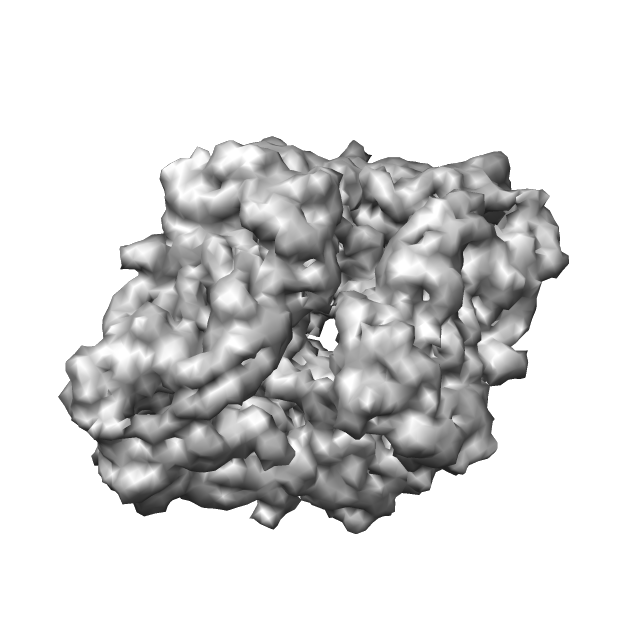
\includegraphics[width=0.5\textwidth]{images/betagal.png}

\vfill % Fill the rest of the page with whitespace
%\begin{minipage}{0.4\textwidth}
\begin{flushright}
 \large
%\emph{Author:}\\
  \textsc{Scipion Team} % Your name
\end{flushright}
%\end{minipage}

\end{titlepage}


%----------------------------------------------------------------------------------------
%	OBJETIVOS
%----------------------------------------------------------------------------------------


\subsection*{Intended audience}

This tutorial presents a general image processing workflow to obtain
3D models of macromolecular complexes using Electron Microscopy (EM).
It is designed to demonstrate how to combine
different EM software packages in Scipion. No prior knowledge is required
about Scipion, but some basic knowledge about 3DEM image processing is asumed
and basic computer skills.

\subsection*{We'd like to hear from you}

We have tested and verified the different steps described in this demo
to the best of our knowledge, but since our programs are in continuous
development you may find inaccuracies and errors in this text. Please
let us know about any errors, as well as your suggestions for
future editions, by writing to
\href{mailto:scipion@cnb.csic.es}{scipion@cnb.csic.es}.

\newpage


%----------------------------------------------------------------------------------------
%	TABLE OF CONTENTS
%----------------------------------------------------------------------------------------

\tableofcontents % Include a table of contents

\newpage % Begins on a new page instead of on the same page as the table of contents


\section{Software Installation}

To follow this tutorial you will need to have \scipion properly installed
in your system. To do so, you can execute the following commands:

%TODO: how to add multiline commands?
\begin{verbatim} 
git clone https://github.com/biocompwebs/scipion.git
cd scipion
./scipion install -j 5
\end{verbatim}

You will also need to install other EM software packages like: 
CTFFind, Spider, Relion, Eman. For the full documentation please refer to the
\href{http://scipion.cnb.csic.es/docs/bin/view/TWiki/NewInstallation}{Scipion installation page}.


\section{Reconstruction of beta-galactosidase}

In this demo, we use the \emph{single particle analysis (SPA)}  approach to obtain
a 3D reconstruction of \emph{beta-galactosidase}. It uses the same test data set than
in Relion 1.3 tutorial, which is subset of the micrographs used in various beta-galactosidase reconstructions \citep{Chen2013, Sjors2012, Vinothkumar2014}.
To reduce
the computational load, these data were 2x down-sampled.


\subsection{Getting Started}

The test data may be downloaded and unpacked using the following commands:

\begin{verbatim}
wget ftp://ftp.mrc-lmb.cam.ac.uk/pub/scheres/relion13_tutorial.tar.gz
gunzip relion13_tutorial.tar.gz
tar -xf relion13_tutorial.tar
\end{verbatim}

After downloading the test data, we will create a project with the workflow pre-loaded
by typing the following command:

\begin{command}
 scipion tutorial betagal
\end{command}

The project windows should appears as shown in Figure \ref{fig:Project}. The previous command has done two 
steps: (1) create a new project. (2) import an existing workflow template. In this way, 
we have a basic template that will made easier to follow the processing pipeline. 

\tipnote{The ability to export/import workflows in \scipion is a great way to 
reproduce previous processing steps. It is particularly useful to repeat steps
on similar samples or to share knowledge between experimental users.}

In the project windows, the left panel displays a tree with the processing tasks (protocols) that 
can be used. The protocols shown can be filtered by perspective (SPA is the default one) or found by Ctrl + F.
Top right panel displays the sequence of protocols executed (runs) by the user and its state: running, finished, aborted. 
Users can visualize the runs in a list or tree views. Finally, bottom right panel displays information for the selected run, 
such as inputs and outputs, execution logs or documentation.
The special \keys{Analyze Results} button can be used to visualize outputs and plot results.

\begin{figure}[H]
\centering
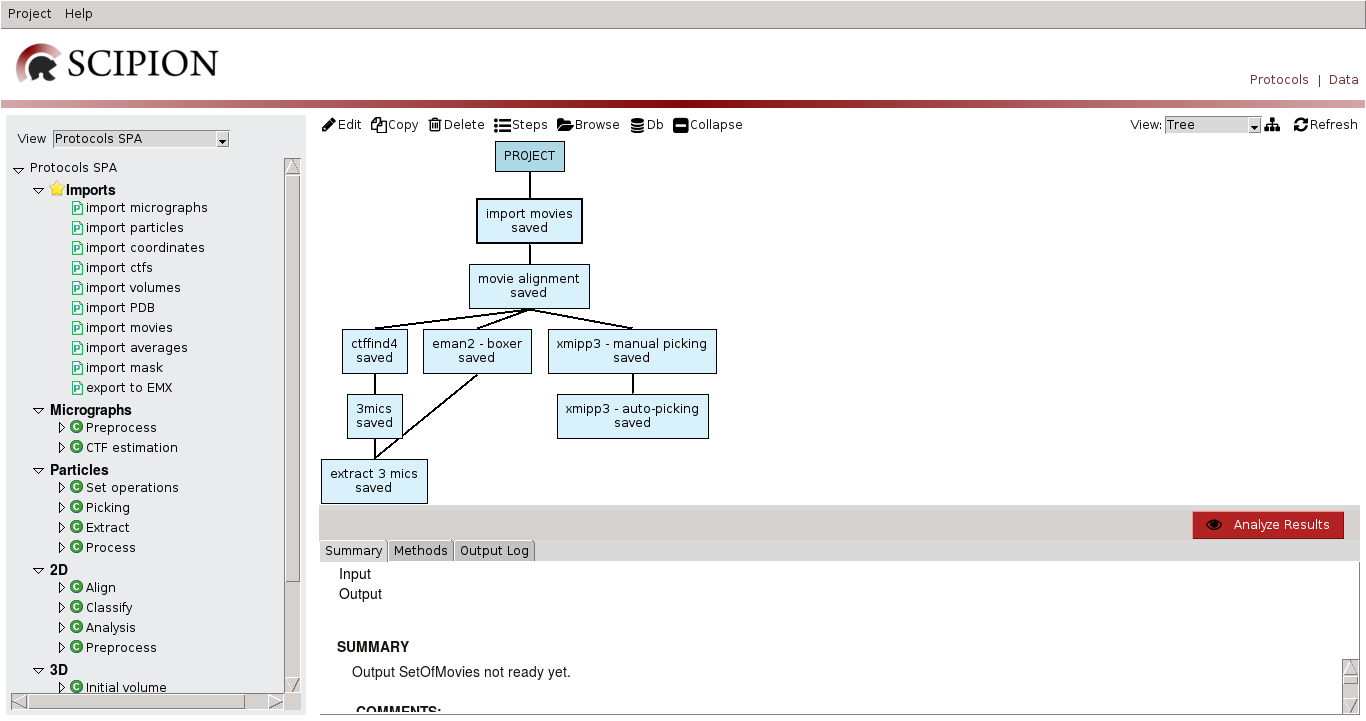
\includegraphics[width=0.9\textwidth]
{{images/00.Project}.png}
\caption{Project window}
\label{fig:Project}
\end{figure}


\subsection{Importing Data and Preprocessing}

In \scipion the \emph{import} is almost the only place where the user needs to deal
directly with files. In our model, each protocol have a very well defined 
inputs and outputs, which are data objects. These objects (SetOfMovies, SetOfParticles, Volume, CTFModel, etc)
encapsulate the underlying files and formats. 

When importing data, like SetOfMovies, SetOfMicrographs or SetOfParticles, the user provides
critical information (such as the Pixel Size). This information will not be requested
any more and will be properly propagated.

\tipnote{Since important information is provided during the \emph{import} step, it is recommended
to take your time to check that all provided parameters are correct. When importing, the binary files
are not copied to the project to avoid data duplication. Instead, a soft link is created pointing 
to the file locations. If you move your project to another computer these links may be broken. There 
is an advanced option where you can set \emph{Copy files?} to Yes. The project is more self-contained
at the price of using more disk space.}


\subsubsection{Movies import}
With the development of the direct electron detectors (DD) low-dose images obtained by electron cryo-microscopy (cryo-EM)
are recorded as frames of movies. The DD have confirmed that the beam-induced motion (BIM) of the sample substantially degrades resolution.
In this section we will show how to import movies and align them to correct the BIM using a combination of global and local movement 
corrections.

To import the movie files, double-click the \keys{import movies} box. The protocol form will be open to fill the paremeters
as shown in Figure \ref{fig:ImportMovs}. In this case, the right values for all the acquisition parameters have been loaded
from the template. Then, we only need to provide the path to the movies files from the downloaded Relion 1.3 data set.
You can either use the \keys{Browse} icon to select the path or type in the entry field.

After selecting the path to the movies, we can press the \keys{Execute} button. This operation should be very fast
since it only search for the files inside the path that match the selected pattern and register a new SetOfMovies
with the provided acquisition information. After executed, the \keys{import movies} box should become green and 
the status should be \emph{finished}. Moreover, the summary tab should display some information such as the number
of movies imported. Now we can click on the \keys{Analyze Results} button and check the list of movies as shown in Figure \ref{fig:MovsList}.
We can right-click in any entry and select \keys{Open} to visualize all the frames in that movie.

\begin{figure}[H]
\centering
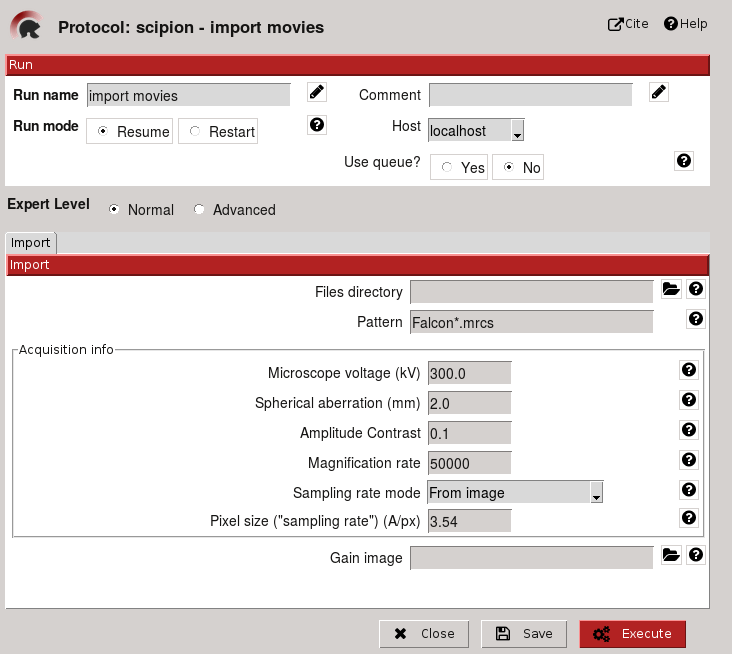
\includegraphics[width=0.7\textwidth]
{{images/01.Import_Movs}.png}
\caption{Import Movies protocol. In this case, only the path needs to be filled.}
\label{fig:ImportMovs}
\end{figure}

\begin{figure}[H]
\centering
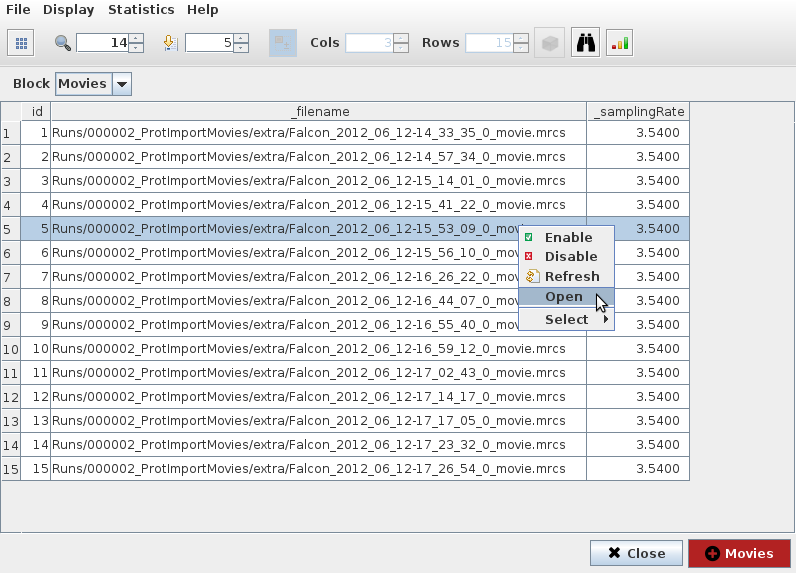
\includegraphics[width=0.9\textwidth]
{{images/02.MovsList}.png}
\caption{Visualization of the resulting set of movies. We can open each movie and visualize its frames. }
\label{fig:MovsList}
\end{figure}

\subsubsection{Movies alignment}
Aligning the individual frames of movies is necessary to correct the BIM image blurring 
and restore important high resolution information. In \scipion we have develop a protocol
that combines both the global and local alignment to produce the final averaged micrograph.

The alignment method used in \citep{Li2013} consists of a pure inplane drift correction in 
which a step of the sub-frame translational alignment is introduced by dividing each frame into a number of
sub-frames This approach is fast if running on GPUs, and at the end, an ‘‘average’’ micrograph is generated for each
movie via the summation of all corrected frames. The method is certainly appropriate for global sample movements
but is not the best option if the sample motion is local. 

The alignment method proposed in \citep{Abrishami2015} is based on Optical Flow (OF) and works best at a local level 
and is therefore particularly suited for those cases in which the BIM pattern presents a high degree of local movements, as in the Falcon II data.
If the BIM pattern is characterized primarily by global movements, OF will have only a minor effect on the final average. 
Still, even for those latter cases, we have found it advantageous to use the \citep{Li2013} method combined with OF,
to obtain an additional level of refinement and a highly intuitive graphical representation of the total BIM pattern.

In our workflow, we can now open the \keys{movie alignment} box (Figure \ref{fig:MovAlignment}) and, since the parameters are filled,
we can execute the protocol. In a general case, we can use the \keys{Search} icon to select the SetOfMovies to be used as input (the options
to select are the objects of this type registered. No more files selection at this point.). In this tutorial we have choose to use \emph{optical flow}
only to be able to used with/without GPU. If the latter is available, then we can try combining both \emph{dosefgpu + optical flow}.
We can also select to exclude some frames from the alignment process.

When finished, we can again click on the \keys{Analyze Results} button. to see the list of the resulting micrographs (Figure \ref{fig:MovAnalyze}).
The first column should be a composite image with half of the PSD of the unaligned micrograph and half of the PSD of the aligned one.
The two plots reflects the average shifts between each pair of frames. The plot in polar coordinates helps to evaluate the magnitude of the movements
while the one in cartesian represents better the direction. The name of each resulting micrographs appears in the last column and can also be opened to 
visual inspection. This protocol should produce as output a new \emph{SetOfMicrographs} that will serve as input to further processing steps.

\begin{figure}[H]
\centering
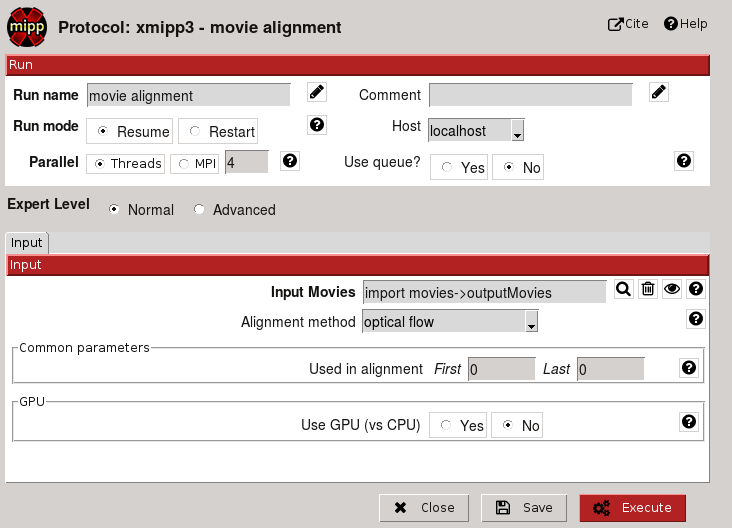
\includegraphics[width=0.7\textwidth]
{{images/03.MovAlignment}.png}
\caption{Movie alignment Protocol. }
\label{fig:MovAlignment}
\end{figure}

\begin{figure}[H]
\centering
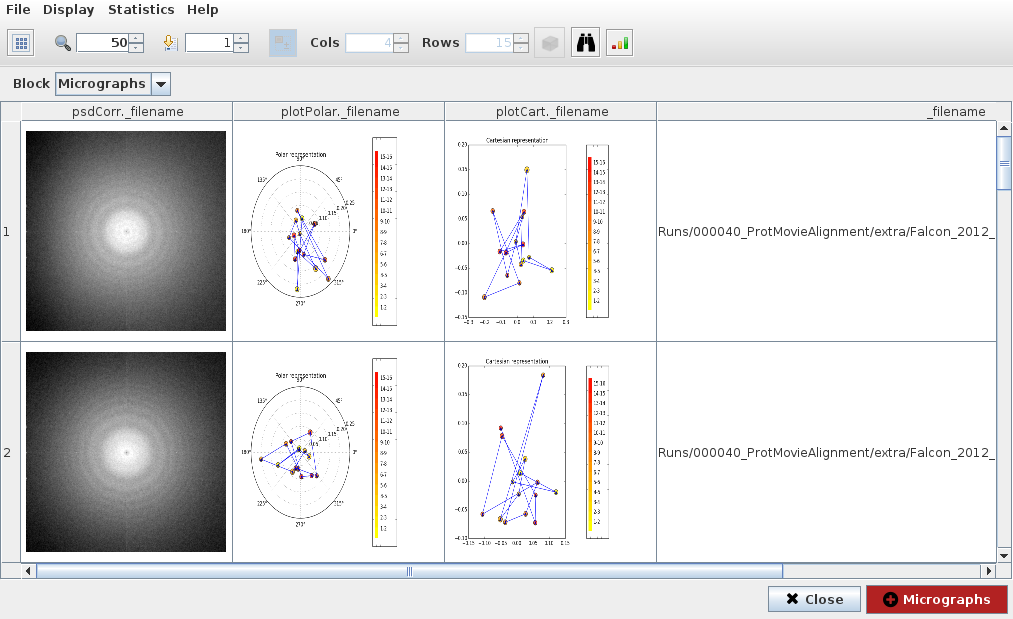
\includegraphics[width=0.9\textwidth]
{{images/04.MovAnalyze}.png}
\caption{Visualization of the Movie alignment outputs. }
\label{fig:MovAnalyze}
\end{figure}

\subsubsection{Micrographs import}
If you already have your movies aligned, then it is possible to import directly the micrograph data.
The import form is very similar to the one for movies. The main different is that for micrograph 
we could import also from \href{http://i2pc.cnb.csic.es/emx}{EMX} format and from Xmipp 3 metadata.
In these cases, CTF information can also be associated with the micrographs. After importing micrographs
we should have an output \emph{SetOfMicrographs} (the same type of output from the movie alignment)
that can be used in further steps.


\subsubsection{Micrographs preprocessing}

Another useful protocol in \scipion is \keys{preprocess - micrographs} which combines multiple 
Xmipp 3 programs in order to perform different operations over the micrographs (Figure \ref{fig:MicPreprocess}).
Depending on the micrographs, sometimes is necessary perform some preprocessing operations such us: reduce 
the micrograph size (usually referred as \emph{downsampling} or \emph{binning}), crop some pixels from the borders
or remove bad pixels applying a filtering operation. In the protocol form we can select the input micrographs
and the operations to perform and execute as usual. The result should be a new \emph{SetOfMicrographs} with 
the transformations applied.

\begin{figure}[H]
\centering
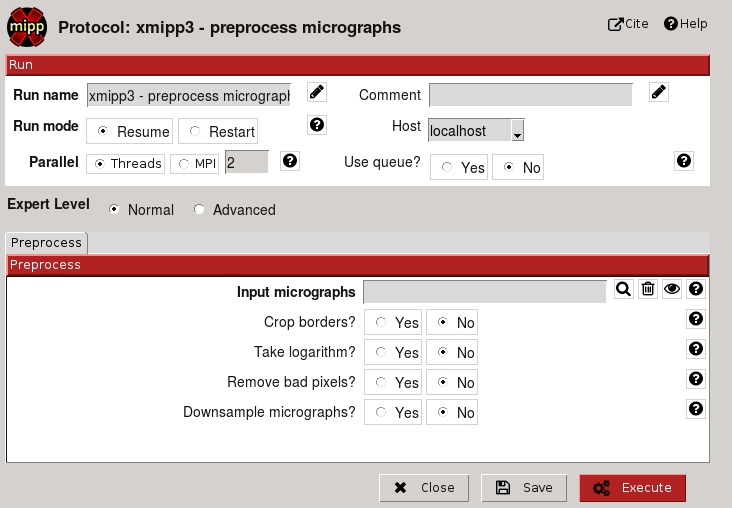
\includegraphics[width=0.7\textwidth]{{images/05.MicPreprocess}.png}
\caption{Preprocess Micrographs Protocol.}
\label{fig:MicPreprocess}
\end{figure}

\subsection{Estimating CTF}

\subsubsection{Using CTFFind and Xmipp}

The next step is to estimate the CTFs (Contrast Transfer Functions) of
the micrographs either using \textit{CTFFind} \citep{Mindell2003} or
\textit{Xmipp CTF estimation} (cite). These protocols estimate the PSD (Power Spectral Density) of the
micrographs and the parameters of the CTF (defocus U, defocus V, defocus angle, etc).  They cut the micrographs into plenty
of images with the desired window size. After that, they compute the Fourier
Transform of each image and make an average.

We have develop the protocols for CTFFind and Xmipp in such a way that the 
parameters are very similar. To estimate the CTF you will need select the frequency region
to be analyzed (Figure \ref{fig:CTFFind}). 
The limiting frequencies must be such that all zeros of the PSD are
contained within those frequencies. There is a wizard, shown in Figure
\ref{fig:CTFWizard}, that helps in choosing those frequencies. To
see the full available options, choose the \emph{Advanced} expert level
and click on the \keys{Help} button for an specific parameter.
The CTFFind protocol allows to use either ctffind3 or ctffind4 programs,
the lastest have been reported to be like ten times faster.

\begin{figure}[H]
\centering
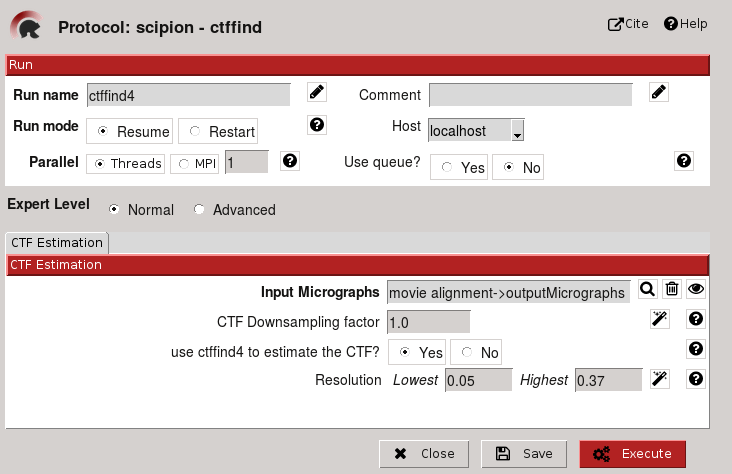
\includegraphics[width=0.7\textwidth]{{images/06.CTFFind}.png}
\caption{CTFFind protocol}
\label{fig:CTFFind}
\end{figure}

\begin{figure}[H]
\centering
  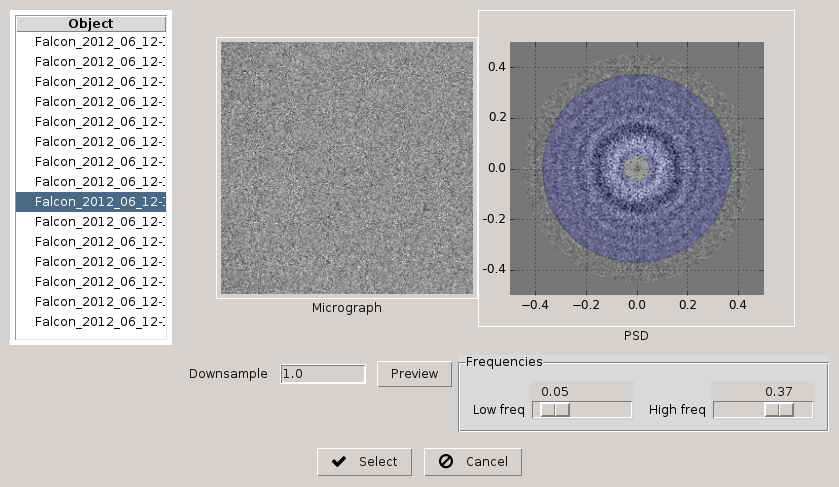
\includegraphics[width=0.7\textwidth]{{images/07.CTFWizard}.png}
  \caption{Wizard to help selecting the frequency region.}
  \label{fig:CTFWizard}
\end{figure}

\subsubsection{Analyzing CTF results}

The CTFs of good micrographs typically have multiple concentric rings, shown
in Figure \ref{fig:CTFs} left, extending from the image center towards its edges.
Bad micrographs may lack rings or have very few rings that hardly extend from
the image center. A reason to discard micrographs may be the presence of
strongly asymmetric rings (astigmatism, Figure \ref{fig:CTFs} center) or rings
that fade in a particular direction (drift, Figure \ref{fig:CTFs} right).

\begin{figure}[H]
\centering
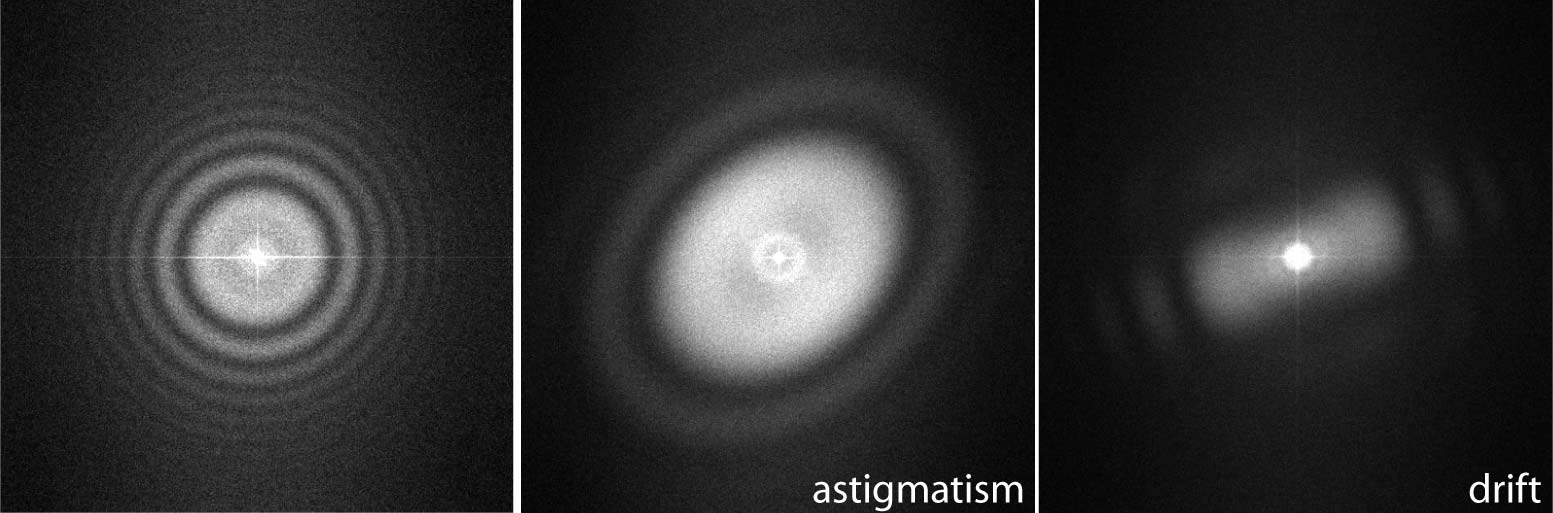
\includegraphics[width=0.75\textwidth]{images/images-016.jpg}
\caption{CTFs of good, astigmatic and drift micrographs respectively.}
\label{fig:CTFs}
\end{figure}

When the protocol (either CTFFind or Xmipp CTF estimation) is finished
you may click on the \keys{Analyze Results} button (Figure
\ref{fig:CTFResult}). To discard micrographs with bad CTFs you may
click with the mouse right button and press \textbf{Disable}. Once you
finish the selection, press on the \keys{Micrographs} button to
create a subset of micrographs with only the enabled ones. 

\tipnote{The creation of user selected subsets is tracked in \scipion
as another operation, so this action is stored in the project workflow.
In the EM packages this kind of operations is usually done by editing
the metadata files, but the action is not longer tracked.}

Sometimes the CTF estimation algorithm may fail to find the rings even
if they can be seen by eye. If this is the case, you may help the
algorithm to find the rings by clicking on the image with the mouse
right-button and choosing \textbf{Recalculate CTF} on the menu that
appears. A graphical interface will help you to correctly identify the
CTF. You must provide the first CTF zero and the search range, and then
press \verb+OK+. When you finish, press the \keys{Recalculate CTFs}
button.

It is also possible to analyze the CTF profiles by right-click on a micrograph row
and selecting the \emph{Show CTF profile} option which should open a windows
as shown in Figure \ref{fig:CTFProfile}. The profile for the Xmipp CTF estimation
show some additional options such as the Envelop. In the CTFFind case, there is
an option to show the CTF fitting as shown in Figure \ref{fig:CTFFitting}.

\begin{figure}[H]
\centering
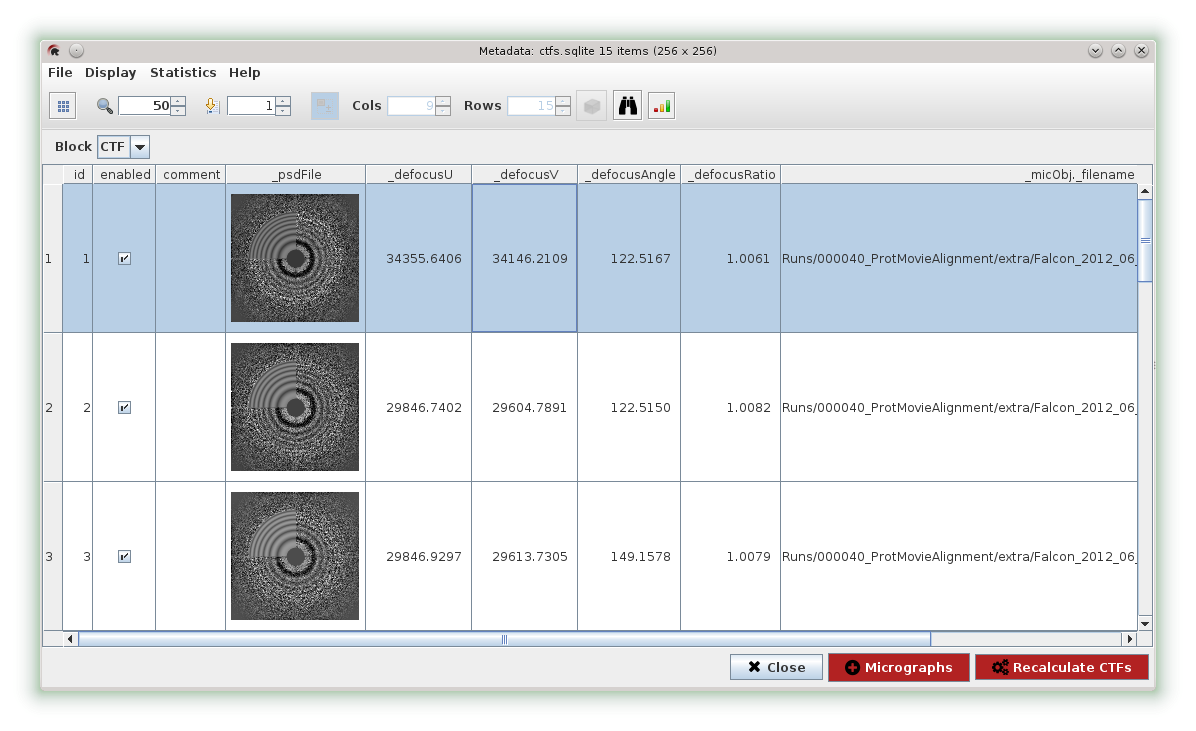
\includegraphics[width=0.9\textwidth]{{images/08.CTFResult}.png}
\caption{Protocol CTFFind output that shows the estimated CTFs for all micrographs.}
\label{fig:CTFResult}
\end{figure}

\begin{figure}[H]
\centering
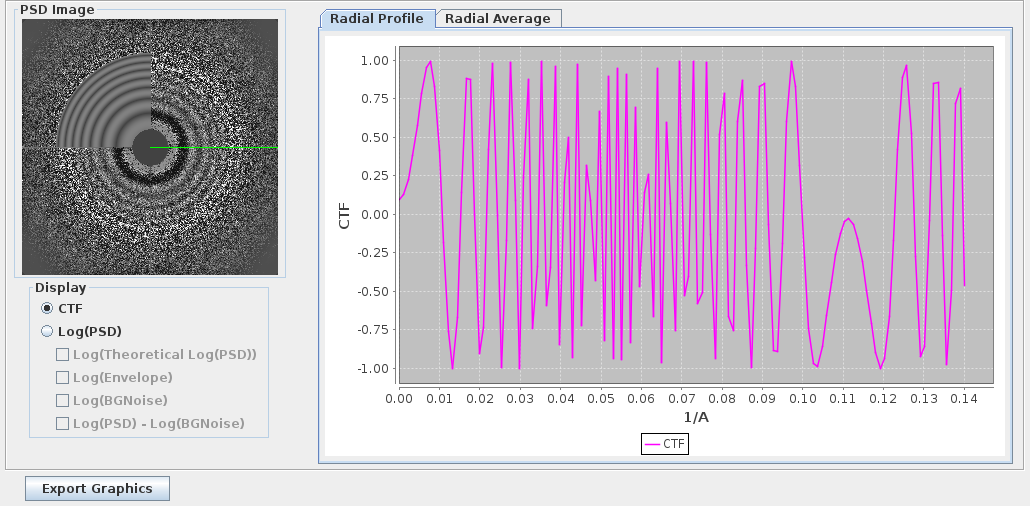
\includegraphics[width=0.7\textwidth]{{images/09.CTFProfile}.png}
\caption{Protocol CTFFind output that shows the estimated CTFs for all micrographs.}
\label{fig:CTFProfile}
\end{figure}

\begin{figure}[H]
\centering
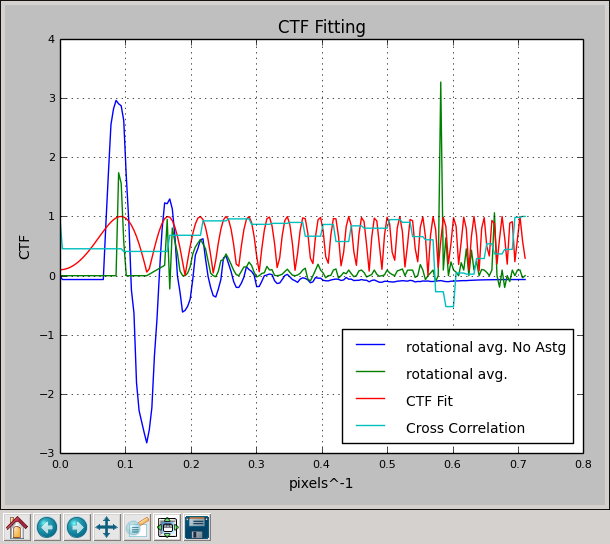
\includegraphics[width=0.6\textwidth]{{images/10.CTFFitting}.png}
\caption{Protocol CTFFind output that shows the estimated CTFs for all micrographs.}
\label{fig:CTFFitting}
\end{figure}

\subsection{Particle Picking}

Particle picking is an important step to select your ''particles'' from the micrograph images.
Manual picking can be very tedious and each tool is more or less convenient depending on 
the sample and the personal preferences. In \scipion, we have integrated different 
picking tools, so the user can select which one better fits its needs, or combine some of them to 
obtain the final coordinates. Currently, the following tools are available:
Eman boxer, Xmipp supervised/automatic, Appion DoG picker, Sparx Gaussian (packaged with Eman), 
Relion autopick and Bsoft manual picking. In this section we will illustrate the usage
of some of them.


\subsubsection{Using Eman boxer}
In this tutorial, before launching the Eman boxer, we will select a subset of 3 micrographs.
To do so, we can open the results from the CTF estimation, order the micrographs by defocus
and select one at the top, one at the middle and one at the end. We can register this new
subset and put a meaningful name that can be easily remembered. This small set will be used
later during Relion picking.

Eman boxer has manual picking and several modes of
automatic picking, with fast outcome. Please refer to its
\href{http://blake.bcm.edu/emanwiki/EMAN2}{webpage} for futher
information. 

We need to open the \keys{eman - boxer} box and executed it, after that we should see the 
boxer GUI as in Figure. For this tutorial we will use a box size of 64 pixels and the 
Swarm tool.

\begin{figure}[H]
\centering
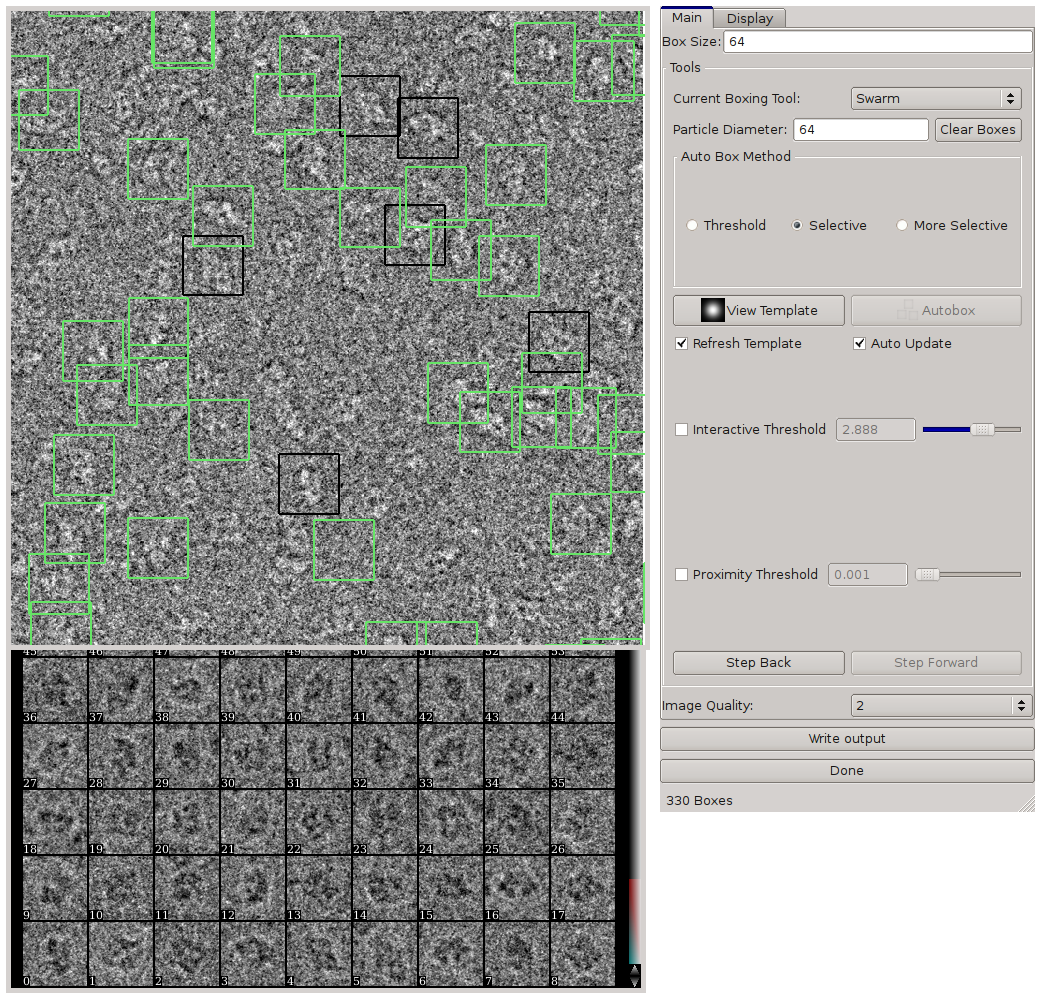
\includegraphics[width=0.9\textwidth]{{images/11.EmanBoxer}.png}
\caption{EMAN boxer, an interface for particle picking.}
\label{fig:EmanBoxer}
\end{figure}

After finished with picking particles with one micrograph, we can move to the next one
and pick all of this small set. At the end, we can click in the \keys{Done} button
in the Boxer GUI and then a dialog should appears asking to register the output
in the project. After that, a \emph{SetOfCoordinates} should appears as output
of this run in the Summary tab.

\subsubsection{Using Xmipp picking}

Xmipp particle picking is divided in two steps: (1) manual/supervised picking and (2) completed automatic
picking. For the manual supervised picking, we open the \keys{xmipp3 - manual picking} box, select the 
input micrographs and execute it. This box will become light yellow, what means that is interactive job
that we can relaunch any time. 

The Xmipp picking GUI (Figure \ref{fig:XmippPick}) contains a control panel with the list of micrographs
and some other parameters. The micrograph where we are picking is displayed in a separated window and
we can apply a number of filters/enhancements (like Gaussian blurring, Invert contrast, adjust histogram)
just to improve the visualization of particles and its selection. Following is a summary of the control
actions:

\begin{itemize}
\item Use \keys{\shift + mouse wheel} in the overview window to zoom
  in and out.
\item Mark particles with the \keys{mouse left} button. You may move
  its position by clicking the left mouse button on the selected
  particle and dragging it to the new position.
\item Use \keys{\shift + left mouse} over a selected particle in order
  to remove it.
\item You can apply filters to the micrographs, so that you may see
  the particles better. Select in the menu \menu{Filters} as many filters
  as you like.
\end{itemize}

\begin{figure}[H]
\centering
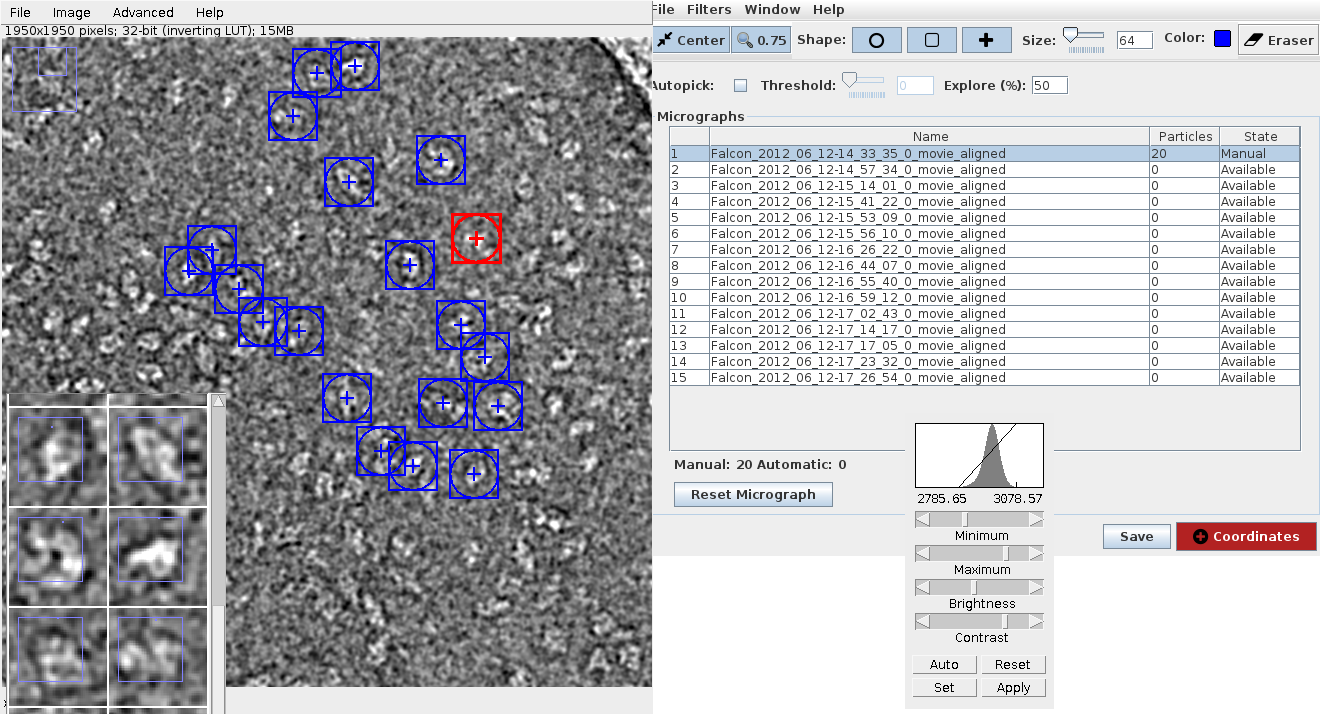
\includegraphics[width=0.9\textwidth]{{images/12.XmippPick}.png}
\caption{Xmipp picking interface.}
\label{fig:XmippPick}
\end{figure}

In the manual/supervised step, we should start picking manually a few micrographs and then mark the \emph{Autopick}
checkbox. At this point, it will train a classifier based in machine learning and will propose some coordinates
automatically. You can ''correct'' the classifier by adding missing particles or removing wrongly picked. 
After training with a few more micrographs, we can register the output coordinates by clicking on the \keys{Coordinates}
red button.

Then we can close the GUI and open the \keys{xmipp3 - automatic} box and select the previous execution of 
manual/supervised as input. When executing, this will pick the rest of micrographs completely automatic.
At the end, we can review the picking coordinates and we still have the chance to add/remove particles.

\tipnote{Once we have trained the classifier in the manual/supervised step, we can even pick another
set of micrographs of new collected data in an automatic fashion.}

\subsubsection{Using Sparx Gaussian}
The Sparx Gaussian picking tool is packaged into Eman. In this picking, we only need to adjust a few
paramters and it will picking particles based on a Gaussian distribution of what is considered particle.
In that sense, it reduce the introduced bias by our eyes or our conception of what is particle.

To use this picking, we can open another Eman boxer run and then select the Gaussian tool. 
After adjusting the parameters for a few micrographs, we should click on the \keys{Done} button, answer yes to 
register the output and it will pick all the input micrographs.

\subsubsection{Using Appion DoG picker}
The Appion DoG picker is based on a difference of gaussians and works in a similar way of the Sparx gaussian.
This picking tool have not GUI, so we should try with some parameters and later visualize the picked coordinates
using the Xmipp GUI. 

\subsubsection{Using Relion auto-picking}
The protocols for Relion auto-picking in \scipion have been divided in two steps: (1) computing the figure-of-merit (FOM) maps and (2)
Adjusting the parameter and picking the rest of the micrographs. The Relion picker is based on a template matching approach, so it
needs to have some 2D averages to search for particles. So you will need to go a bit ahead to the 2D section and produce some classes
and go back to Relion and use them as references. 

In the first step, the FOM maps are written to disc for just a few micrographs, which are recommended to be representative of your whole
data set(high and low-defocus one, and/or with thin or thick ice). Then in the second step, there is a wizard, which will launch again
the Relion program but now reading the previous FOM maps in order to speed up the computation. On this way, adjusting the parameters becomes
more interactive. After we are happy with the results for this few micrographs, we can then launch the auto-picking for the full set 
of micrographs in a completed automatic way. When finished, we can again review the output particles with the Xmipp GUI and add/remove
particles.

\subsubsection{Extracting Particles}

Once we have any set of coordinates, we can proceed to extract these particles with Xmipp.
We need to be careful with the options selected here, since this will affect later steps.
The extract protocol (Figure \ref{fig:XmippExtract}) will allow us 
to extract, normalize and correct the CTF phase of your picked
particles, among other things. The options are summarized below:

\begin{itemize}
\item The \textit{coordinates} of the particles in the micrographs,
  which are taken from the results of the previous step. Also in the
  same tab, the \textit{particle box size} in pixels (in this case 64
  px).
\item The \textit{invert contrast} flag. If activated, bright
  regions become dark regions and the other way around. 

\item The \textit{phase flipping} flag. If activated,
  the protocol corrects the CTF phase of your particles. 

\item The \textit{normalize} flag. If activated (recommended), the
  particles are normalized to have zero mean and a standard deviation
  of one for the background pixels.
\end{itemize}

\begin{figure}[H]
\centering
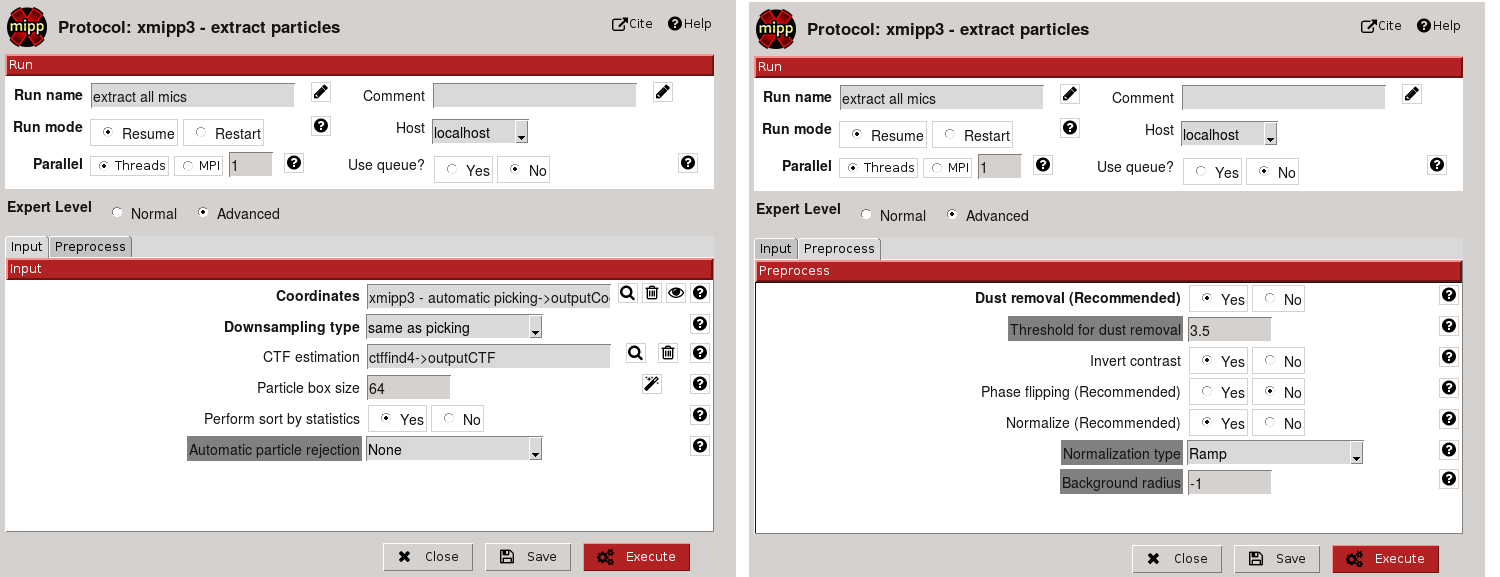
\includegraphics[width=0.9\textwidth]{{images/13.XmippExtract}.png}
\caption{Extract particles protocol. Available options are shown.}
\label{fig:XmippExtract}
\end{figure}

% TODO: see the definition of zscore and explain this a bit more.

In this case, we have choose to invert the contrast, since we will use 
Relion later for 2D and 3D classification, and it expects the particles
to be white over black. In the case of Frealign, it expect the particles 
on the other way, black over white. We have also choose not to do phase 
flipping, because Relion also likes to handle that correction internally.
If we were going to use some Xmipp programs in the later steps, it is 
recommended to do phase flipping here.

We have also checked the \emph{Sort by statistics} option, which 
tell the protocol to sort the particles based on general statistics
assigning to each particle a z-score value. Particles with low z-score
are reliable and the ones with large z-score are outliers. Press the
\keys{Analyze Results} button in the main window to check the
extracted and normalized images (Figure \ref{fig:XmippExtract2} and \ref{fig:XmippExtract3}). 
If the \emph{Sort by statistics} was 
checked, the particles will be sorted (ascending) by the z-score value
and the z-score will also be plot. If you want to remove some particles, eg: because they are outliers, you can use 
\menu{right click > disable }.
To create a new set of particles you can click on \keys{Particles} red button.

\begin{figure}[H]
\centering
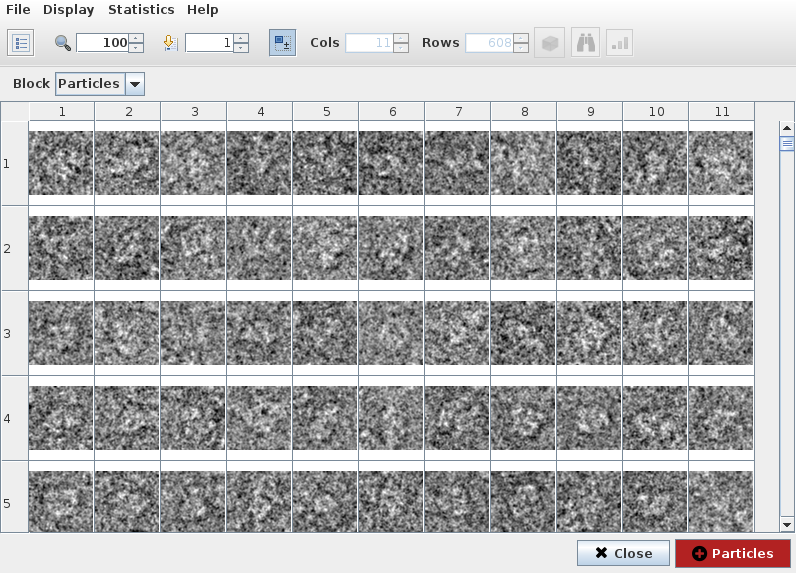
\includegraphics[width=0.8\textwidth]{{images/13.XmippExtract2}.png}
\caption{List of particles after extraction, sorted by z-score.}
\label{fig:XmippExtract2}
\end{figure}

\begin{figure}[H]
\centering
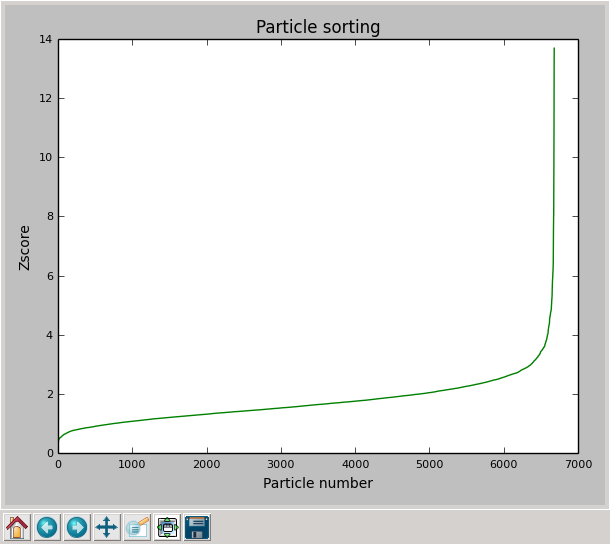
\includegraphics[width=0.7\textwidth]{{images/13.XmippExtract3}.png}
\caption{Plot of the z-score values.}
\label{fig:XmippExtract3}
\end{figure}

\tipnote{The GUI to visualize particles can be used with other protocols to create subsets based on some quality parameter.
Particles can be easily ordered by any column and then make selection base on that order to discard bad particles.}
\subsection{3D Reconstruction: Projection Matching}

Having the right angles of each projection is crucial for making a 3D
reconstruction.  However, in 3DEM you don’t know a priori the angles
and you have to estimate them as part of the problem. The most popular
way of estimating them is by comparing somehow the projections of a
volume that is similar to the volume to be reconstructed (initial
model) with the images obtained from the microscope.

A possible approach is to generate equidistant projections from the
initial model. The experimental dataset is then compared (for
example, by cross correlation) to each reference projection.  A
“similarity” coefficient (for example, crosscorrelation coefficient)
is generated between each experimental particle and reference
projection. Each individual experimental particle is matched to the
reference projection that gave the highest “similarity”
coefficient. Therefore, it is assumed that this experimental particle
was projected with the same Euler angles as the reference projection.

As an initial map is necessary, we provide initial volume. Click on 
\menu{Imports > Import Volume} and import from

% TODO: explain where. Which dialog? which menu?
% Maybe it's \menu{3D > Preprocess > xmipp3 - preprocess volumes}
% but I don't know.

% TODO: acutally, from this point below (and the last paragraph), it
% is not clear where to click on things, or how the flow is going. I
% think it should be revisited.


\begin{verbatim}
$SCIPION_HOME/data/tests/xmipp_tutorial/micrographs/
\end{verbatim}

\noindent volume \comm{BPV\_scale\_filtered\_windowed\_110.vol} with \textit{sampling rate} 6.185.

To run the projection matching protocol click on
\menu{3D > Refine > xmipp3 -projection matching} and choose expert mode.
Input parameters are displayed in Figures \ref{fig:ProjMatchA}, \ref{fig:ProjMatchB},
\ref{fig:ProjMatchC} and \ref{fig:ProjMatchD} . Here we explain only the ones we need to update
for this reconstruction. For more detail on each parameter please use the respective 
\textbf{help} button.


 
We need to specify parameters below and execute protocol.
\begin{itemize}
\item \textit{Input particles:} Particles selected previously.
\item \textit{Initial 3D reference volumes:}  Initial volume registered.
\item \textit{Mask reference volumes:} Circular. Masking the reference volume will increase the signal to noise ratio. 
\item \textit{Radius of spherical mask(px):} 55. Since particles size is 110 radius of spherical mask should be 55.
\item \textit{Inner radius for rotational correlation:} 28. Particles will be correlated considering points covered 
by inner and outer radius for rotational correlation.
\item \textit{Outer radius for rotational correlation:} 55. Since particles size is 110 outer radius for rotational correlation should be 55.
\item \textit{Point group symmetry:} i1. Virus type of symmetry.
\item \textit{Constant to be added to the estimated resolution:} -0.05. The volume will be filtered at a frequency equal to
the  resolution computed with resolution\_fsc(FSC=0.5) plus the value provided in this field.

\end{itemize}


Finally, in order to visualize volume reconstructed click on
\keys{Analyze Results} button. Protocol viewer will be displayed (Figure \ref{fig:ProjMatchViewer}).


In the field 
\textit{Display volume with slices } press the \textbf {eye} button and you will see the 
volume slice by slice (Figure \ref{fig:volShowj}). To visualize the volume with chimera select
chimera (Figure \ref{fig:volChimera}).


\subsection{Frealign Refinement}

If you want to refine the output volume of projection matching, you can
use \menu{3D > Refine > grigoriefflab - frealign}. First, you need to process the set of particles
that was used as input for projection matching with the features needed
for frealign.


To do this, extract the particles
again, but preprocess particles as shown in Figure \ref{fig:ExtractForFrealign}.

 
Once the particles are extracted, use \menu{Particles > Set operations > scipion subset}
to create a new set with the particles contained in this set that were used for reconstruction.

Input parameters are displayed in Figures \ref{fig:FrealignA}, \ref{fig:FrealignB}, \ref{fig:FrealignC}
and \ref{fig:FrealignD} . Here we explain only the ones we need to update
for this refinement. 



We need to specify:
\begin{itemize}
\item \textit{Input particles:} Set of particles that was used as input for projection matching 
with the features needed for frealign.
\item \textit{Initial 3D reference volumes:}  Projection matching output volume
\item \textit{Reconstruction radius:} Inner, 10. Outer, 315. Inner and outer radius of the volume to be reconstructed.
\item \textit{Point group symmetry:} I1. Virus symmetry
\item \textit{Resolution of reconstruction:} 15. Resolution to which the reconstruction is calculated.
\item \textit{Resolution in refinement:} Low, 200. High, 20. Resolution of the data included in the search/refinement.
\item \textit{High resolution for classification:} 20. Resolution of the data included in the search/refine. It should typically be set to the same resolution
limit used for the refinement.

\end{itemize}
Then we execute the protocol.


Finally we have obtained the 3D reconstruction of a \emph{Bovine Papillomavirus}.
In order to visualize volume refined click on \keys{Analyze Results}
button or open output volume registered.
Figure \ref{fig:FrealignViewer}.

 
We hope this tutorial was of use to you as a general introduction to Scipion.
Our goal is to allow the users like you to execute workflows combining different software tools, while taking care of formats and conversions. 



\bibliographystyle{apalike}
\bibliography{../tutorial_common/em.bib}

\end{document}
